\chapter{Evaluation and Interpretability}
\label{ch:eval}

\chapmeta{Advanced}{$\sim$4\,h (2\,h + 2\,h)}{LoveDA; trained checkpoints}

\begin{objbox}
\begin{itemize}[leftmargin=1.2em,nosep]
  \item Define and compute IoU, mIoU, Dice, pixel accuracy and per-class F1.
  \item Build and correctly normalise a confusion matrix for segmentation.
  \item Apply GradCAM to see where a CNN ``looks''.
  \item Use prediction-entropy maps to flag uncertain regions.
  \item Conduct a structured failure analysis and propose targeted fixes.
\end{itemize}
\end{objbox}

A land-cover map is only as trustworthy as its evaluation. This chapter
formalises the metrics used throughout the course and adds interpretability
tools that turn ``the mIoU is 0.58'' into actionable understanding of \emph{where}
and \emph{why} the model fails.

\section{Segmentation metrics}

Let TP, FP, FN be the per-class pixel counts. The \emph{Intersection over Union}
(Jaccard index) for class $k$ and its mean over classes are
\begin{equation}
\mathrm{IoU}_k = \frac{\mathrm{TP}_k}{\mathrm{TP}_k+\mathrm{FP}_k+\mathrm{FN}_k},
\qquad
\mathrm{mIoU} = \frac{1}{K}\sum_{k=1}^{K}\mathrm{IoU}_k.
\label{eq:iou}
\end{equation}
mIoU is the standard segmentation headline because, unlike pixel accuracy, it
weights every class equally and is not inflated by a dominant background. The
\emph{Dice} (F1) coefficient is closely related,
\begin{equation}
\mathrm{Dice}_k = \frac{2\,\mathrm{TP}_k}{2\,\mathrm{TP}_k+\mathrm{FP}_k+\mathrm{FN}_k}
= \frac{2\,\mathrm{IoU}_k}{1+\mathrm{IoU}_k},
\end{equation}
always at least as large as IoU and more forgiving of small errors
(Figure~\ref{fig:iou}). \emph{Pixel accuracy} (fraction of correctly labelled
pixels) is reported for completeness but is misleading under class imbalance.

\begin{figure}[h]
\centering
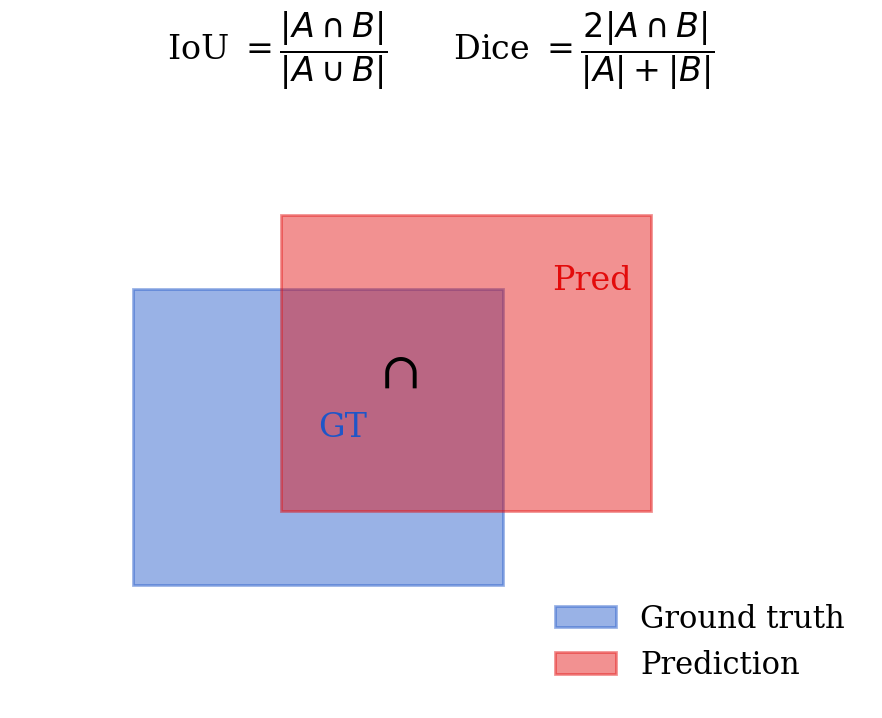
\includegraphics[width=0.62\linewidth]{figures/iou.png}
\caption{IoU and Dice for a predicted region (red) versus ground truth (blue).
IoU divides intersection by union; Dice doubles the intersection over the sum of
areas. Both reward overlap and penalise both false positives and false
negatives.}
\label{fig:iou}
\end{figure}

\section{The confusion matrix}

The $K\times K$ confusion matrix $C$, with $C_{ij}$ the number of pixels of true
class $i$ predicted as $j$, is the richest single diagnostic. \emph{Row-normalise}
it ($C_{ij}/\sum_j C_{ij}$) to read per-class recall and to see which classes are
confused for which (Figure~\ref{fig:cm}). In land cover the off-diagonal mass
concentrates among semantically adjacent classes --- grassland vs agriculture,
urban vs bare soil --- which points directly at where extra bands, indices or
augmentation would help.

\begin{figure}[h]
\centering
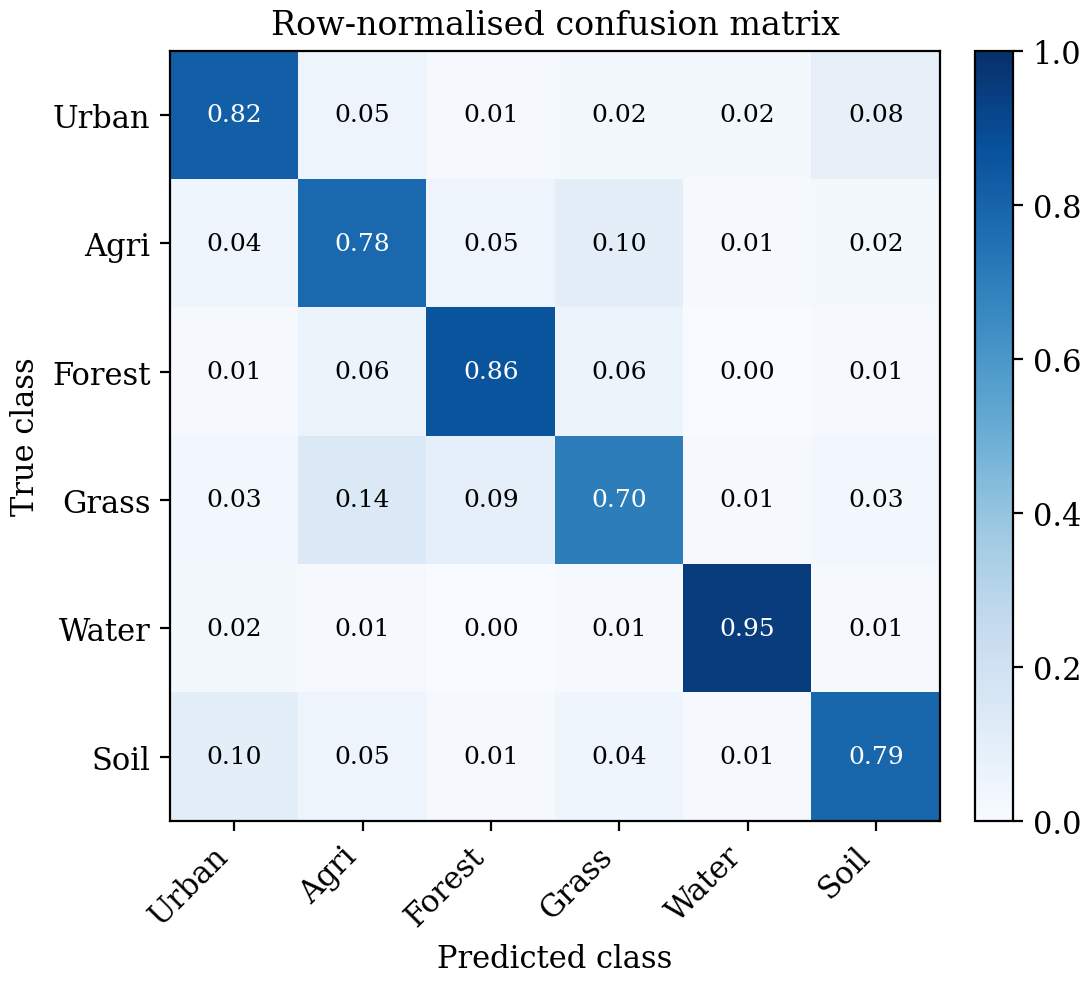
\includegraphics[width=0.52\linewidth]{figures/confusion.png}
\caption{Row-normalised confusion matrix. The diagonal is per-class recall;
bright off-diagonal cells (e.g.\ grassland $\to$ agriculture) reveal systematic,
explainable confusions to target.}
\label{fig:cm}
\end{figure}

\section{GradCAM: what the model sees}

GradCAM produces a coarse heat-map of the image regions most responsible for a
prediction. For target class $c$ and the activations $A^{k}$ of a chosen
convolutional layer, the neuron-importance weights are the
gradient-global-average
\begin{equation}
\alpha^{c}_{k} = \frac{1}{Z}\sum_{i,j}\frac{\partial y^{c}}{\partial A^{k}_{ij}},
\qquad
L^{c}_{\mathrm{GradCAM}} = \mathrm{ReLU}\!\Big(\sum_{k}\alpha^{c}_{k} A^{k}\Big),
\end{equation}
upsampled to the input size. For EO it answers questions like ``did the network
classify this patch as \textsf{Industrial} because of the buildings or because of
an adjacent road?'', exposing spurious correlations (a model keying on image
borders or compression artefacts is a real failure mode).

\section{Uncertainty via entropy}

The per-pixel predictive entropy of the softmax distribution,
\begin{equation}
\mathcal{H}(\mathbf{p}) = -\sum_{k=1}^{K} p_k \log p_k,
\end{equation}
is a cheap uncertainty proxy: high entropy marks pixels where the model hedges
--- typically class boundaries and genuinely ambiguous land cover. An entropy
\emph{map} overlaid on the prediction shows reviewers exactly where to look and
is the basis of active-learning sample selection.

\section{Failure analysis}

Good practice closes the loop: rank validation tiles by error, inspect the worst,
categorise the mistakes (boundary leakage, whole-class confusion, rare-class
misses, tiling seams), attribute each to a cause, and propose a targeted fix
(class weighting for rare classes, more overlap for seams, extra indices for
spectral confusion). A short, honest discussion of failure cases is what
separates a portfolio project from a toy --- and is explicitly rewarded in the
capstone rubric.

\begin{keybox}
\begin{itemize}[leftmargin=1.2em,nosep]
  \item mIoU (Eq.~\ref{eq:iou}) is the class-balanced headline; pixel accuracy misleads under imbalance.
  \item Dice $\ge$ IoU; both penalise FP and FN.
  \item Row-normalised confusion matrices reveal \emph{which} classes are confused.
  \item GradCAM localises evidence; entropy maps localise uncertainty.
  \item Structured failure analysis turns metrics into targeted improvements.
\end{itemize}
\end{keybox}

\begin{practbox}
Notebook: \nbpath{chapter\_12\_evaluation\_interpretability/12\_practical\_evaluation\_interpretability.ipynb}.
\begin{enumerate}[leftmargin=1.4em,nosep]
  \item Implement per-class IoU, mIoU, Dice, pixel accuracy and F1 from a confusion matrix.
  \item Plot a publication-quality row-normalised confusion matrix.
  \item Apply GradCAM to a trained model for selected classes; interpret the heat-maps.
  \item Compute and visualise a prediction-entropy map.
  \item Rank tiles by error and write a short failure-mode report.
\end{enumerate}
\end{practbox}

\begin{exbox}
\textbf{12.1 IoU vs Dice.} Construct prediction/GT pairs where IoU and Dice
disagree most; explain the geometry.\\[2pt]
\textbf{12.2 Boundary metric.} Implement a boundary-IoU that scores only pixels
near class edges; compare with standard IoU.\\[2pt]
\textbf{12.3 Calibration.} Plot a reliability diagram of predicted confidence vs
accuracy; is the model over- or under-confident?\\[2pt]
\textbf{Mini-project.} Build an \texttt{evaluation\_report(model, loader)} that
emits a metrics table, confusion matrix, GradCAM panel, entropy map and a ranked
failure gallery as a single figure/markdown bundle.
\end{exbox}
